\documentclass[tikz,border=2pt]{standalone}
\usepackage{amsmath,amssymb}
\usetikzlibrary{arrows.meta}
\begin{document}
% The four subspaces of an m x n matrix A: A maps the row space Row(A) onto Col(A) and Null(A) to 0;
% A^+ undoes A from Col(A) back onto the row space and sends Null(A^T) to 0.
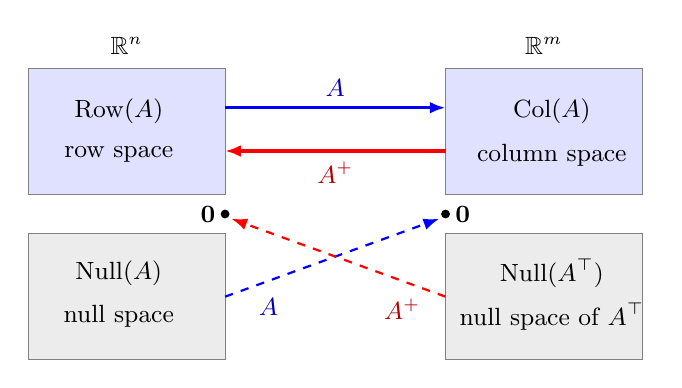
\begin{tikzpicture}[font=\small, >={Latex[length=2mm]}]
  % domain R^n
  \fill[blue!12] (0,0.25) rectangle (2.5,1.85);
  \fill[gray!15] (0,-1.85) rectangle (2.5,-0.25);
  \draw[gray] (0,0.25) rectangle (2.5,1.85);
  \draw[gray] (0,-1.85) rectangle (2.5,-0.25);
  \node at (1.15,1.3) {$\operatorname{Row}(A)$};
  \node at (1.15,0.75) {row space};
  \node at (1.15,-0.75) {$\operatorname{Null}(A)$};
  \node at (1.15,-1.3) {null space};
  \node[anchor=south] at (1.25,1.9) {$\mathbb{R}^n$};
  \fill (2.5,0) circle (1.6pt) node[left] {$\boldsymbol{0}$};
  % codomain R^m
  \fill[blue!12] (5.3,0.25) rectangle (7.8,1.85);
  \fill[gray!15] (5.3,-1.85) rectangle (7.8,-0.25);
  \draw[gray] (5.3,0.25) rectangle (7.8,1.85);
  \draw[gray] (5.3,-1.85) rectangle (7.8,-0.25);
  \node at (6.65,1.3) {$\operatorname{Col}(A)$};
  \node at (6.65,0.75) {column space};
  \node at (6.65,-0.75) {$\operatorname{Null}(A^{\top})$};
  \node at (6.65,-1.3) {null space of $A^{\top}$};
  \node[anchor=south] at (6.55,1.9) {$\mathbb{R}^m$};
  \fill (5.3,0) circle (1.6pt) node[right] {$\boldsymbol{0}$};
  % row space <-> column space
  \draw[->, blue, very thick] (2.5,1.35) -- (5.3,1.35) node[midway, above, blue!70!black] {$A$};
  \draw[->, red, very thick] (5.3,0.8) -- (2.5,0.8) node[midway, below, red!70!black] {$A^+$};
  % null spaces to zero
  \draw[->, blue, thick, dashed] (2.5,-1.05) -- (5.22,-0.06);
  \node[blue!70!black, anchor=north] at (3.05,-0.95) {$A$};
  \draw[->, red, thick, dashed] (5.3,-1.05) -- (2.58,-0.06);
  \node[red!70!black, anchor=north] at (4.75,-0.95) {$A^+$};
\end{tikzpicture}
\end{document}
